\documentclass[12pt, a4paper]{article}
\edef\restoreparindent{\parindent=\the\parindent\relax}
\usepackage[utf8]{inputenc}
\usepackage[T1]{fontenc}
\usepackage{XCharter}
\usepackage{amsmath}
\usepackage[UKenglish]{babel}
\usepackage[bibstyle=ieee, dashed=false, sorting=nty]{biblatex}
\usepackage[labelfont=bf]{caption}
\usepackage{csquotes}
\usepackage{fancyhdr}
\usepackage{float}
\usepackage[top=25mm, right=25mm, bottom=20mm, left=25mm]{geometry}
\usepackage{graphicx}
\usepackage[hidelinks]{hyperref}
\usepackage{microtype}
\usepackage{multicol}
\usepackage{parskip}
\usepackage{titlesec}
\usepackage{xparse}

\restoreparindent

\pagestyle{fancy}
\fancyhead[L]{COM4506}
\fancyhead[C]{Assignment: Metamorphic Testing}
\fancyhead[R]{160203853}
\setlength{\headheight}{15pt}

\setcounter{secnumdepth}{4}

% \titleformat{\paragraph}
% {\normalfont\normalsize\bfseries}{Category \Alph{subsubsection}\arabic{paragraph}}{1em}{}
% \titlespacing*{\paragraph}{0pt}{3.25ex plus 1ex minus .2ex}{1.5ex plus .2ex}

% \newcounter{category}[subsubsection]
% \newcommand{\category}[2]{\stepcounter{category} \textbf{Category #1\thecategory: #2} \par}

\newcounter{category}[subsection]
\newenvironment{category}[3][]{\refstepcounter{category}\par\medskip
\noindent \underline{\textbf{Category~#1\thecategory \quad #2}} \rmfamily\par #3}{\bigskip}

\addbibresource{references.bib}

\begin{document}

\setlength{\abovedisplayskip}{0pt}
\setlength{\abovedisplayshortskip}{0pt}

\section{Category Partition Method}

%----------------------------------------------------------------------------------------
%	List
%----------------------------------------------------------------------------------------
\subsection{Parameter: List}
\begin{category}[L]{Empty list}
  \textbf{Input:} \texttt{list = []}
  \par
  \textbf{Reason:} One of the edge cases of the \texttt{List} interface. Given this as the input,
  both \texttt{Collections.sort} and \texttt{Collections.rotate} should return an empty list as the
  output.
\end{category}

\begin{category}[L]{Single element in the list}
  \textbf{Input:} \texttt{list = [$x$]}, where $x$ is an element of a class that implements the
  \texttt{Comparable} interface.
  \par
  \textbf{Reason:} One of the edge cases of the \texttt{List} interface. The output returned by both
  \texttt{Collections.sort} and \texttt{Collections.rotate} should be the same as the input.
\end{category}

\begin{category}[L]{More than one element in the list}
  \textbf{Input:} \texttt{list = [$x_0, x_1, \dots, x_n$]} for $n > 1$, where $n$ is the number of
  elements in the list, and $x_0, x_1, \dots, x_n$ are the elements of a class that implements the
  \texttt{Comparable} interface.
  \par
  \textbf{Reason:} The is the minimum viable test case for testing the actual functionality of
  \texttt{Collections.sort} and \texttt{Collections.rotate}. This is the base form that is used to
  define other variants of the input (\textbf{Category L4 - L7}).
\end{category}

\begin{category}[L]{Duplicate elements in the list}
  \textbf{Input:} \texttt{list = [$x_0, x_1, \dots, x_n$]} for $n > 1$. The list follows the input
  restrictions of \textbf{Category L3}. \textbf{N.B.} In addition, there also exists some $\{a, b\}
  \in n$ where the value of $x_a$ is equal to $x_b$.
  \par
  \textbf{Reason:} This is to test whether the \texttt{Collections.sort} method is able to handle
  duplicate elements. The duplicate elements should be arranged next to each other in the sorted
  list.
\end{category}

\begin{category}[L]{List is in random order}
  \textbf{Input:} \texttt{list = [$x_0, x_1, \dots, x_n$]} for $n > 1$. The list follows the input
  restrictions of \textbf{Category L3}, but the list is could be arranged in a way where $x_k <
  x_{k+1}$, but $x_{k+2} < x_k$ for all $k \in n$. The list can also contain duplicate elements.
  \par
  \textbf{Reason:} This is to test the sorting capability of \texttt{Collections.sort}. It is
  expected that the input will be sorted into ascending order, according to the natural ordering of
  its elements.
\end{category}

\begin{category}[L]{List is in ascending natural order of its elements}
  \textbf{Input:} \texttt{list = [$x_0, x_1, \dots, x_n$]} for $n > 1$. The list follows the input
  restrictions of \textbf{Category L3}, and the list can contain duplicate elements. However, the
  list must be arranged according to the natural ordering \cite{java_natural_order} of its elements,
  where $x_0 \leq x_1,\  x_1 \leq x_2,\  \dots,\  x_{n-1}$
  \par
  \textbf{Reason:} This is to test the sorting consistency of \texttt{Collections.sort}. Since the
  input list is already sorted, then sorting the input list should return a list then is arranged in
  the same order as the input list.
\end{category}

\begin{category}[L]{List is in descending natural order of its elements}
  \textbf{Input:} \texttt{list = [$x_0, x_1, \dots, x_n$]} for $n > 1$. The list follows the input
  restrictions of \textbf{Category L3}, and the list can contain duplicate elements. However, the
  list must be arranged according to the \textbf{reverse} natural ordering \cite{java_natural_order}
  of its elements, where $x_0 \geq x_1,\  x_1 \geq x_2,\  \dots,\  x_{n-1} \geq x_n$.
  \par
  \textbf{Reason:} This is the inverse test case of \textbf{Category L6}, where the input list is
  sorted in reverse order. The aim is to ensure that \texttt{Collections.sort} can handle the cases
  where certain parts of the list (i.e. sub-list) are inversely sorted.
\end{category}

\begin{category}[L]{List size is greater than or equal to \texttt{ROTATE\_THRESHOLD}}
  \textbf{Input:} \texttt{list = [$x_0, x_1, \dots, x_n$]} for $n \geq \texttt{ROTATE\_THRESHOLD}$,
  where the value of \\\texttt{ROTATE\_THRESHOLD} is defined as 100 in \texttt{Collections.java}
  \cite{rotate_threshold_variable}.
  \par
  \textbf{Reason:} According to the source code of \texttt{Collections.java}
  \cite{rotate_threshold_branch}, Java uses two different algorithm to rotate lists that are < or
  $\geq$ than \texttt{ROTATE\_THRESHOLD} respectively. The aim is to validate that both algorithms
  are able to correctly rotate the input list.
\end{category}

%----------------------------------------------------------------------------------------
%	distance
%----------------------------------------------------------------------------------------
\subsection{Parameter: distance}
\begin{category}[D]{Negative number}
  \textbf{Input:} \texttt{distance < 0}
  \par
  \textbf{Reason:} To ensure that the \texttt{Collections.rotate} method will work with negative
  distance input by covering the negative domain of \texttt{int} data type.
\end{category}

\begin{category}[D]{Zero}
  \textbf{Input:} \texttt{distance == 0}
  \par
  \textbf{Reason:} 0 is the default value of \texttt{int} data type in Java, and also the starting
  index value of \texttt{List}. This is to ensure that the \texttt{Collections.rotate} method will
  work when the input distance is zero.
\end{category}

\begin{category}[D]{Positive number}
  \textbf{Input:} \texttt{distance > 0}
  \par
  \textbf{Reason:} To ensure that the \texttt{Collections.rotate} method will work with positive
  distance input by covering the positive domain of \texttt{int} data type.
\end{category}

\begin{category}[D]{Smaller than list size}
  \textbf{Input:} \texttt{distance < list.size()}
  \par
  \textbf{Reason:} A stricter variant of \textbf{Category D1 - D3}.
\end{category}

\begin{category}[D]{Equal to list size}
  \textbf{Input:} \texttt{distance == list.size()}
  \par
  \textbf{Reason:}
\end{category}

\begin{category}[D]{Larger than list size}
  \textbf{Input:} \texttt{distance > list.size()}
  \par
  \textbf{Reason:} A stricter variant of \textbf{Category D3}.
\end{category}

\begin{category}[D]{Equal to minimum boundary value of \texttt{int}}
  \textbf{Input:} \texttt{distance ==} $-2^{31}$
  \par
  \textbf{Reason:} The minimum value an \texttt{int} can have in Java is $-2^{31}$
  \cite{int_min_value}. The aim is to validate the assumption that if \texttt{Collections.rotate}
  works for the minimum value of \texttt{int}, then it should work correctly for any value larger
  than the minimum value.
\end{category}

\begin{category}[D]{Equal to maximum boundary value of \texttt{int}}
  \textbf{Input:} \texttt{distance ==} $2^{31} - 1$
  \par
  \textbf{Reason:} The maximum value an \texttt{int} can have in Java is $2^{31} - 1$
  \cite{int_max_value}. The aim is to validate the assumption that if \texttt{Collections.rotate}
  works for the maximum value of \texttt{int}, then it should work correctly for any value smaller
  than the maximum value.
\end{category}

%----------------------------------------------------------------------------------------
%	Collection
%----------------------------------------------------------------------------------------
\subsection{Parameter: Collection}
\begin{category}[C]{Single element in collection}
  \textbf{Input:}
  \par
  \textbf{Reason:}
\end{category}

\begin{category}[C]{More than one element in collection}
  \textbf{Input:}
  \par
  \textbf{Reason:}
\end{category}

\begin{category}[C]{Duplicate elements in collection}
  \textbf{Input:}
  \par
  \textbf{Reason:}
\end{category}

\begin{category}[C]{Duplicate minimum elements in collection}
  \textbf{Input:}
  \par
  \textbf{Reason:}
\end{category}

\begin{category}[C]{Collection is in random order}
  \textbf{Input:}
  \par
  \textbf{Reason:}
\end{category}

\begin{category}[C]{Collection is in ascending natural order of its elements}
  \textbf{Input:}
  \par
  \textbf{Reason:}
\end{category}

\begin{category}[C]{Collection is in descending natural order of its elements}
  \textbf{Input:}
  \par
  \textbf{Reason:}
\end{category}


\section{Test Cases}

\subsection{\texttt{Collections.sort(List<T> list)}}

\subsection{\texttt{Collections.rotate(List<?> list, int distance)}}

\subsection{\texttt{Collections.min(Collection<? extends T> coll)}}

\section{Metamorphic Relations}
% \begin{figure}[H]
%   \centering
%   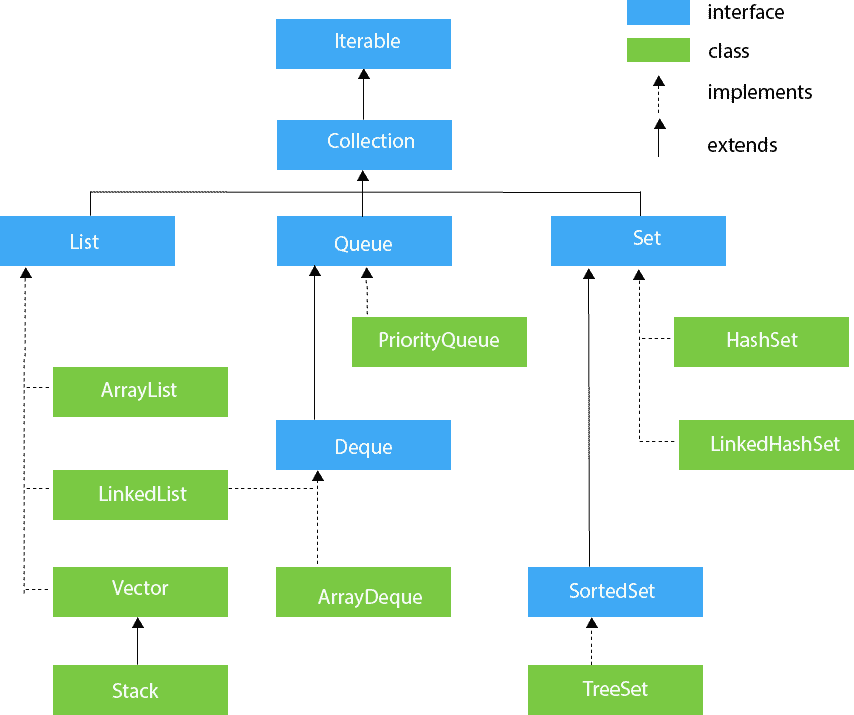
\includegraphics[width=.75\textwidth]{images/java-collection-hierarchy.png}
%   \caption{Java Collections Framework hierarchy \cite{java_collection_hierarchy}.}
% \end{figure}


\section{Remarks}


\printbibliography

\end{document}
